\documentclass[12pt]{article}
\usepackage{amsmath}
\usepackage{amssymb}
\usepackage{amsthm}
\usepackage{amsfonts}
\usepackage{graphicx}
\usepackage{textcomp}
\usepackage{hyperref}
\usepackage{tikz}
\usepackage{enumitem}
\usepackage{mathtools}
\usepackage{enumitem}
\usepackage{wasysym}
\usepackage{ulem}
\usepackage{xspace}
\usepackage{csquotes}
\usepackage{booktabs}

\DeclareMathOperator{\dist}{dist}
\DeclareMathOperator{\Nul}{Nul}
\DeclareMathOperator{\Row}{Row}
\DeclareMathOperator{\proj}{proj}

\setlength{\arraycolsep}{12pt}

\newcommand{\defn}{\textbf{Def.}\xspace}
\newcommand{\thm}{\textbf{Thm.}\xspace}
\newcommand{\ex}{\textbf{ex.}\xspace}
\newcommand{\Ex}{\textbf{Ex.}\xspace}
\newcommand{\ie}{\textbf{i.e.}\xspace}
\newcommand{\lemma}{\textit{Lemma}\xspace}
\newcommand{\bproof}{\textit{Proof ($\impliedby$).}\xspace}
\newcommand{\fproof}{\textit{Proof ($\implies$).}\xspace}
\newcommand{\bigEps}{\mathcal{E}}
\newcommand{\soln}{\textit{Soln.}\xspace}

\renewcommand{\arraystretch}{1.25} % Adjust row spacing


\hypersetup{
    colorlinks=true,
    linkcolor=blue,
    filecolor=blue,      
    urlcolor=blue,
}

\newcommand{\ulhref}[2]{\href{#1}{\color{blue}\uline{#2}}}

\begin{document}

\title{MACM 316 Lecture 23 - Chapter 3 Part 2}
\author{Alexander Ng}
\date{Monday, March 10, 2025}

\maketitle

\section*{Lecture Review}

In this lecture, he begins with a review of somet things that we covered in
lecture 22 and 21, which he was absent for and had a TA teach for him.

\subsection{Divided Differences}

Assume that $f(x)$ is known at several points along the x-axis. We do not assume
that the $x$'s are evenly spaced or even that the values are arranged in any
particular order.

We write the (any arbitrary) $n^{th}$ degree polynomial in the following way:

\[
  P_n(x) = a_0 + a_1 (x-x_0) + a_2 (x-x_0) (x-x_1) + \dots + a_n (x-x_0) \dots (x-x_{n-1})
.\]

\defn $P_n(x)$ is an interpolating polynomial for $f(x)$ at $x_0, x_1, \dots, x_n$
if we choose $a_i$ such that $P_n(x) = f(x))$ at the $n+1$ known points.

We want to find our $a_i$ to make $P_n(x)$ an interpolating polynomial, and we
can determine our $a_I$ by using what are called the \enquote{divided
differences.}

\subsubsection{The Zeroth Divided Difference}

First, we determine $a_0: P_n(x_0) = f(x_0) = a_0$, and define the
$\text{zero}^{\text{th}}$ (degree) divided difference as

\[
  f[x_i] = f(x_i)
,\]

\noindent
which is just the value of $f$ at $x_i$.

\subsubsection{The First Divided Difference}

Now we need to determine $a_1$:

\[
P_n(x_1) = f(x_1) = a_0 + (x_1 - x_0) a_1
.\]

Rearranging, we get

\[
a_i = \frac{f(x_1) - f(x_0)}{x_1 - x_0} = \frac{f[x_1] - f[x_0]}{x_1 - x_0}
.\]

which allows us to determine $a_1$ by using the $\text{zero}^{\text{th}}$ 
divided difference. We define the first divided difference of $f$ with respect
to $x_i$ and $x_{i+1}$ as

\[
  f[x_i, x_{i+1}] = f[x_{i+1}, x_i] = \frac{f[x_{i+1}]-f[x_i]}{x_{i+1}-x_i}
.\]


\subsubsection{The Second Divided Difference}

Similarly, the second divided difference is defined as 

\[
  f[x_i, x_{i+1}, x_{i+2}] = \frac{f[x_{i+1}, x_{i+2}] - f[x_i, x_{i+1}]}{x_{i+2}-x_i}
.\]

\subsubsection{The Kth Divided Difference}

In a similar fashion to the evaluation of $a_0$ and $a_1$, we can show

\[
  a_k = f[x_0, x_1, \dots, x_k]
.\]

This gives Newton's Interpolatory divided difference formula

\begin{align*}  
  P_n(x) &= f[x_0] + f[x_0, x_1] (x-x_0) \\
         &\quad+ f[x_0, x_1, x_2] (x-x_0) (x-x_1) \\
         &\quad+ \dots \\
         &\quad+ f[x_0, x_1, \dots, x_n](x-x_0) \dots (x-x_{n-1})
\end{align*}

\subsubsection{Disadvantages of Divided Differences}

\begin{itemize}
\item $P_n(x)$ could be expensive to evaluate
\item $P_n(x)$ does go through the datapoints, but between each datapoint, we
  could have large oscillations, which we expect as the generic behaviour of
  large degree polynomials.
  \subitem This is especially true near endpoints, where our datapoints are
  sparse and sections where our function is not smooth.
\end{itemize}

\section{Better Interpolating Polynomials - Ch2. Pt3. (14.1)}

The Lagrange Polynomial can oscillate wildly, except where contained between
datapoints that are in close proximity. We want our interpolating polynomial to
have the same \enquote{shape} as the function at the datapoints. In other words,
we want the tangent lines (first derivative) and the function itself to agree at
$(x_i, f_1)$

\subsection{Proof from (14.2).} 

This section is directly copied from the Chapter 3 Part 2 pdf.

\thm
If \( f \in C^1[a,b] \) and \( x_0, \ldots, x_n \in [a,b] \) are distinct, the interpolating polynomial of least degree agreeing with \( f \) at \( x_0, \ldots, x_n \) is the Hermite polynomial of degree at most \( 2n+1 \) given by

\[
H(x) = \sum_{j=0}^{n} f(x_j) H_j(x) + \sum_{j=0}^{n} f'(x_j) \hat{H}_j(x)
\]

where

\[
H_j(x) = \left[1 - 2(x - x_j)L_j'(x_j)\right] L_j^2(x)
\]

and

\[
\hat{H}_j(x) = (x - x_j) L_j^2(x)
\]

where \( L_j(x) \) denotes the Lagrange coefficient polynomial of degree \( n \).

\begin{proof}
See text for a derivation showing that \( H(x) \) agrees with \( f \) and \( H'(x) \) agrees with \( f' \) at \( x_0, x_1, \ldots, x_n \).

To show the uniqueness of this polynomial:

Suppose that \( P(x) \) is another polynomial with
\[
P(x_{j}) = f(x_{j}), \quad P'(x_{j}) = f'(x_{j}) \quad \text{for } j = 0, \ldots, n
\]
and that the degree of \( P(x) \) is at most \( 2n+1 \).

Let \( D(x) = H(x) - P(x) \). Then \( D(x) \) is a polynomial of degree at most \( 2n+1 \).

The zeros at each \( x_0, x_1, \ldots, x_n \) are equal to
\[
D(x) = (x - x_0)^2 \cdots (x - x_n)^2 Q(x)
\]

Either \( D(x) \) is of degree \( 2n + 2 \) or more, which would be a contradiction, 
\uline{or}
\[
Q(x) \equiv 0 \Rightarrow D(x) \equiv 0 \Rightarrow P(x) = H(x)
\]
which implies that the polynomial is unique.
\end{proof}

\subsection{The Newton Interpolatory divided difference formula}

Unfortunately, a direct application of the theorem requires us to evaluate the
Lagrange Polynomials and their derivatives, which is tedious even for small
values of $n$. Instead, we use the Newton Interpolatory divided difference
formula:

Select a new sequence of nodes $z_0, z_1, \dots, z_{2n+1}$ 

\[
  z_{2i} = z_{2i+1} = x_i
.\]

We have a small problem. 

\[
  f[z_{2i}] = f[z_{2i+1}] = f(x_i)
.\]

\[
  f[z_{2i}, z_{2i+1}] = \frac{f[z_{2i+1}] - f[z_{2i}]}{z_{2i+1} - z_{2i}}
.\]

This gives us $\frac{0}{0}$, which is not defined. Instead, we think of taking
the limit as $z_{2i}$ approaches $z_{2i+1}$:

\[
  f[z_{2i}, z_{2i+1}] = \lim_{z_{2i} \to z_{2i+1}} \frac{f[z_{2i+1}] - f[z_{2i}]}{z_{2i+1} - z_{2i}}
.\]

% Which gives the exact formal definition of the first derivitive of $f$ at $z_{2i}$

Thus, the derivative values are used in place of the undefined first divided
differences, otherwise Newton's divided differences are produced as usual.

\begin{center}
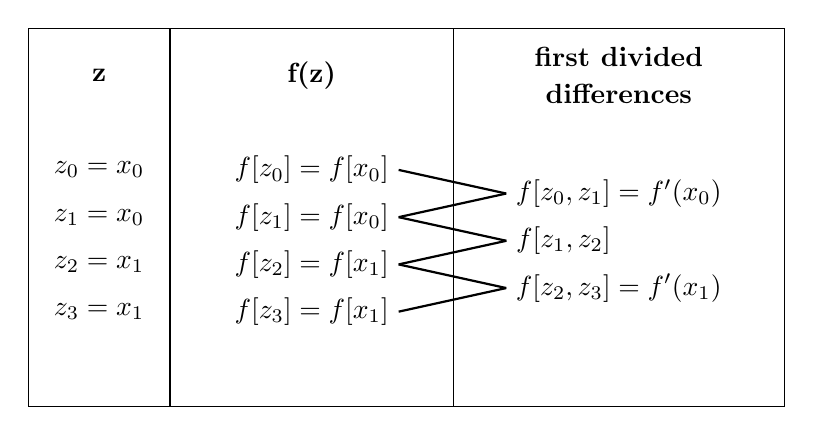
\begin{tikzpicture}[scale=1.2]
\draw (0,0) rectangle (8,4);

% Horizontal lines
% \foreach \y in {1,2,3}
% \draw (0,\y) -- (9,\y);

% Vertical lines
\draw (1.5,0) -- (1.5,4);
\draw (4.5,0) -- (4.5,4);

% Column titles
\node at (0.75,3.5) {\textbf{z}};
\node at (3,3.5) {\textbf{f(z)}};
\node at (6.25,3.7) {\textbf{first divided}};
\node at (6.25,3.3) {\textbf{differences}};
% \node at (8.25,3.7) {\textbf{second divided}};
% \node at (8.25,3.3) {\textbf{differences}};

% Entries for z
\node at (0.75,2.5) {$z_0 = x_0$};
\node at (0.75,2) {$z_1 = x_0$};
\node at (0.75,1.5) {$z_2 = x_1$};
\node at (0.75,1) {$z_3 = x_1$};

% Entries for f(z)
\node (F1) at (3,2.5) {$f[z_0] = f[x_0]$};
\node (F2) at (3,2) {$f[z_1] = f[x_0]$};
\node (F3) at (3,1.5) {$f[z_2] = f[x_1]$};
\node (F4) at (3,1) {$f[z_3] = f[x_1]$};

% First divided differences
\node (1D1) at (6.25,2.25) {$f[z_0,z_1] = f'(x_0)$};
\node (1D2) at (6.25,1.75) {$f[z_1,z_2]\qquad\qquad$};
\node (1D3) at (6.25,1.25) {$f[z_2,z_3] = f'(x_1)$};

\draw[thick] (F1.east) -- (1D1.west);
\draw[thick] (F2.east) -- (1D1.west);
\draw[thick] (F2.east) -- (1D2.west);
\draw[thick] (F3.east) -- (1D2.west);
\draw[thick] (F3.east) -- (1D3.west);
\draw[thick] (F4.east) -- (1D3.west);

% \draw[thick] (1D1.east) -- (1D2.west);
% \draw[thick] (1D2.east) -- (1D3.west);

% Second divided differences
% \node (2D1) at (8.25,2.25) {$f[z_0,z_1,z_2] = f''(x_0)$};
% \node (2D2) at (8.25,1.75) {$f[z_1,z_2,z_3]$};
% \node (2D3) at (8.25,1.25) {$f[z_2,z_3,z_4] = f''(x_1)$};

% \draw[thick] (F1.east) -- (2D1.west);
% \draw[thick] (F2.east) -- (2D1.west);
% \draw[thick] (F3.east) -- (2D2.west);
% \draw[thick] (F4.east) -- (2

\end{tikzpicture}
\end{center}

\subsection{The Hermite Polynomial}

The Hermite polynomial is then defined as

\[
  H(x) = f[z_0] + \sum_{k=1}^{2n+1} f[z_0, \dots, z_k]\prod_{j=0}^{k-1} (x-z_j)
.\]

\section{Splines}

Previously, we saw how to compute an approximation to a function over some
finite interval using a single polynomial. We increased the degree of the
polynomial if we wanted more accuracy.


\end{document}
